\chapter{Chemical Potential and Mixtures}\label{ch:b2:chemical-potential}

In winter a truck spreads salt on an icy road and the ice melts at
\qty{-10}{\celsius}; the coolant of a car engine, water with a third of
ethane-1,2-diol, neither freezes in the night frost nor boils under a hot
bonnet. A dissolved substance lowers the freezing point of its solvent and
raises its boiling point, and, for dilute solutions, by an amount that
depends on the number of dissolved particles and not on what they are. The
tool that explains it is the \omterm{def:b2:chemical-potential:chemical-potential}{chemical potential}, the partial derivative of
the \omterm{def:b2:reaction-free-energy:gibbs-energy}{Gibbs energy} with respect to the amount of one constituent. It tells
where each species ``wants to go'', between phases and through reactions,
and it turns the activities that the Year 1 volume used as recipes into
derived quantities.

\begin{recall}
\Cref{ch:b2:reaction-free-energy}: the \omterm{def:b2:reaction-free-energy:gibbs-energy}{Gibbs energy} $G = H - TS$, $\dd G =
V\dd p - S\dd T + \Delta_r G\,\dd\xi$, the evolution criterion $\Delta_r G\,
\dd\xi \leq 0$. The Year 1 volume wrote the activity of a gas as
$p_i/p^\circ$, of a solute as $c_i/c^\circ$, and 1 for a pure solid or a
solvent, and noted that in concentrated ionic solutions activities depart
from concentrations, ``a correction treated in the Year 2 volume''. From
physics: the perfect-gas law, and $(\partial G/\partial p)_T = V$ for a pure
substance.
\end{recall}

\begin{omfigure}

\includegraphics[width=0.58\linewidth]{images/book3/ai/b2-03-salt-spreader.jpg}

{\small A gritting truck spreads salt on a snowy road. The salt dissolves
in the thin film of water on the ice, and the solution freezes at a lower
temperature than pure water: the ice melts.}
\end{omfigure}

\section{Partial molar quantities}

Mix \qty{50}{mL} of water and \qty{50}{mL} of ethanol: the volume of the
mixture is less than \qty{100}{mL}. In a mixture, an extensive quantity is
not the sum of the contributions of the pure substances; each constituent
contributes according to its surroundings.

\begin{definition}[Partial molar quantity]\label{def:b2:chemical-potential:partial-molar}
Let $X(T, p, n_1, \dots, n_k)$ be an extensive state function of a phase
containing the amounts $n_1, \dots, n_k$. The \emph{partial molar
quantity}\index{partial molar quantity} of constituent $i$ is
\[
  \bar X_i = \left(\frac{\partial X}{\partial n_i}\right)_{T, p, n_{j \ne i}} ,
\]
the change of $X$ per mole of $i$ added to a large amount of the mixture
at fixed $T$, $p$ and other amounts. For $X = V$ it is the \emph{partial
molar volume}\index{partial molar volume} $\bar V_i$.
\end{definition}

\begin{theorem}[Euler's identity]\label{thm:b2:chemical-potential:euler}
At fixed $T$ and $p$, $X = \sum_i n_i\bar X_i$.
\end{theorem}

\begin{proof}
$X$ is extensive: multiplying every amount by $\lambda$ multiplies $X$ by
$\lambda$, $X(T, p, \lambda n_1, \dots, \lambda n_k) = \lambda X(T, p, n_1,
\dots, n_k)$. Differentiate with respect to $\lambda$ at $\lambda = 1$, with
the chain rule: $\sum_i n_i\,\partial X/\partial n_i = X$.
\end{proof}

\begin{proposition}[Gibbs--Duhem relation]\label{prop:b2:chemical-potential:gibbs-duhem}
At fixed $T$ and $p$, $\sum_i n_i\,\dd\bar X_i = 0$: in a binary mixture,
$x_1\dd\bar X_1 + x_2\dd\bar X_2 = 0$. The partial molar quantities of the
constituents cannot vary independently.
\end{proposition}

\begin{proof}
At fixed $T$, $p$, $\dd X = \sum_i\bar X_i\dd n_i$ by definition; Euler's
identity, differentiated, gives $\dd X = \sum_i\bar X_i\dd n_i + \sum_i
n_i\dd\bar X_i$. Subtract.
\end{proof}

\begin{omfigure}
\begin{tikzpicture}
\begin{axis}[
  width=0.62\linewidth, height=5.4cm, xmin=0, xmax=1, ymin=8, ymax=62,
  axis x line=bottom, axis y line=left, xlabel={mole fraction $x_2$},
  ylabel={molar volume $V_m$ (model)}, xtick={0,0.2,0.4,0.6,0.8,1}, ytick=\empty,
  tick label style={font=\small}, label style={font=\small}, ylabel shift=10pt, clip=false]
\addplot[omDef, very thick, domain=0:1, samples=60] {18*(1-x) + 58*x - 25*x*(1-x)};
\addplot[black!40, dashed, domain=0:1] {18*(1-x) + 58*x};
\addplot[omThm, thick, domain=0:1] {14 + 35*x};
\fill[omThm] (axis cs:0.4,28) circle (1.6pt);
\node[omThm, anchor=east, font=\small] at (axis cs:-0.01,14) {$\bar V_1$};
\node[omThm, anchor=west, font=\small] at (axis cs:1,49) {$\bar V_2$};
\node[font=\scriptsize, anchor=south east, black!60] at (axis cs:0.62,44) {pure volumes added};
\node[font=\small, anchor=north west] at (axis cs:0.41,27) {$x_2 = 0.4$};
\end{axis}
\end{tikzpicture}

{\small The tangent construction. The molar volume of a model binary mixture
(blue) lies below the straight line joining the pure volumes: mixing
contracts. The tangent at a composition cuts the two edges at the \omterm{def:b2:chemical-potential:partial-molar}{partial
molar volumes} $\bar V_1$ and $\bar V_2$ of that composition.}
\end{omfigure}

\begin{method}[Partial molar quantities from a curve]\label{met:b2:chemical-potential:tangent}
Plot the molar quantity $X_m = X/(n_1 + n_2)$ against $x_2$. At the
composition of interest draw the tangent: it cuts the axis $x_2 = 0$ at
$\bar X_1$ and the axis $x_2 = 1$ at $\bar X_2$. (Proof: $X_m = x_1\bar X_1 +
x_2\bar X_2$ and, by Gibbs--Duhem, $\dd X_m/\dd x_2 = \bar X_2 - \bar X_1$.)
\end{method}

\section{The chemical potential}

\begin{definition}[Chemical potential]\label{def:b2:chemical-potential:chemical-potential}
The \emph{chemical potential}\index{chemical potential} of constituent $i$ in
a phase is its partial molar \omterm{def:b2:reaction-free-energy:gibbs-energy}{Gibbs energy},
\[
  \mu_i = \left(\frac{\partial G}{\partial n_i}\right)_{T, p, n_{j\ne i}} ,
\]
in \unit{J/mol}. Its value when $i$ is in its standard state is its
\emph{standard chemical potential}\index{standard chemical potential}
$\mu_i^\circ(T)$, equal to the standard molar \omterm{def:b2:reaction-free-energy:gibbs-energy}{Gibbs energy} of $i$.
\end{definition}

For a phase whose amounts can change (by reaction, or by exchange with
another phase),
\[
  \dd G = V\dd p - S\dd T + \sum_i\mu_i\,\dd n_i ,\qquad G = \sum_i n_i\mu_i ,
\]
the second relation by Euler's identity. With a single reaction, $\dd n_i =
\nu_i\dd\xi$, and comparing with \cref{prop:b2:reaction-free-energy:dG}:
\[
  \Delta_r G = \sum_i\nu_i\mu_i .
\]
The \omterm{def:b2:reaction-free-energy:reaction-gibbs}{reaction Gibbs energy} is the balance of the \omterm{def:b2:chemical-potential:chemical-potential}{chemical potentials} of the
products and of the reactants.

\begin{theorem}[Equilibrium between phases]\label{thm:b2:chemical-potential:phase-equilibrium}
A constituent present in two phases $\alpha$ and $\beta$ of a closed system at
uniform $T$ and $p$ is at equilibrium between them if and only if
$\mu_i^\alpha = \mu_i^\beta$. Otherwise it passes spontaneously from the
phase where its \omterm{def:b2:chemical-potential:chemical-potential}{chemical potential} is higher to the phase where it is lower.
\end{theorem}

\begin{proof}
The transfer $i^\alpha \to i^\beta$ is a ``reaction'' with $\nu^\alpha = -1$,
$\nu^\beta = +1$, so $\Delta_r G = \mu_i^\beta - \mu_i^\alpha$. By the
evolution criterion it advances ($\dd\xi > 0$) only if $\mu_i^\beta <
\mu_i^\alpha$, recedes if $\mu_i^\beta > \mu_i^\alpha$, and is at
equilibrium if they are equal.
\end{proof}

The \omterm{def:b2:chemical-potential:chemical-potential}{chemical potential} plays for matter the part that temperature plays
for heat: heat flows from hot to cold, a species from high to low $\mu$.

\section{Ideal systems and activities}

\begin{proposition}[Chemical potential of a perfect gas]\label{prop:b2:chemical-potential:mu-gas}
In a mixture of perfect gases, a gas of partial pressure $p_i$ has
\[
  \mu_i = \mu_i^\circ(T) + RT\ln\frac{p_i}{p^\circ} .
\]
\end{proposition}

\begin{proof}
For one mole of a pure perfect gas, $(\partial\mu/\partial p)_T = V_m =
RT/p$; integrating from $p^\circ$ to $p$ gives $\mu = \mu^\circ + RT\ln(p/p^\circ)$.
In a mixture of perfect gases each gas behaves as if alone in the volume, at
its partial pressure: replace $p$ by $p_i$.
\end{proof}

\begin{definition}[Ideal mixture, ideal dilute solution]\label{def:b2:chemical-potential:ideal-mixture}
A liquid (or solid) mixture is an \emph{ideal mixture}\index{ideal mixture}
if, for every constituent and every composition,
$\mu_i = \mu_i^*(T, p) + RT\ln x_i$, where $\mu_i^*$ is the \omterm{def:b2:chemical-potential:chemical-potential}{chemical potential}
of the pure liquid $i$. A solution is an \emph{ideal dilute
solution}\index{ideal dilute solution} if the solvent obeys this law and each
solute obeys $\mu_j = \mu_j^\circ(T) + RT\ln(c_j/c^\circ)$, with a standard
state that is a hypothetical solution at $c^\circ = \qty{1}{mol/L}$ behaving
as if infinitely dilute.
\end{definition}

Molecules of similar size and shape whose interactions do not depend on
the partner (benzene and toluene, two isotopic forms of a molecule) form
nearly \omterm{def:b2:chemical-potential:ideal-mixture}{ideal mixtures}; dilute solutions behave ideally because each solute
particle is surrounded by solvent alone.

\begin{theorem}[Raoult's law]\label{thm:b2:chemical-potential:raoult}
Above an ideal liquid mixture, with the vapour a perfect gas, the partial
pressure of each constituent is proportional to its mole fraction in the
liquid: $p_i = x_i\,p_i^*$, where $p_i^*$ is the vapour pressure of the pure
liquid at the same temperature (\emph{Raoult's law}\index{Raoult's law}).
\end{theorem}

\begin{proof}
At equilibrium $\mu_i(\text{liquid}) = \mu_i(\text{vapour})$: $\mu_i^* +
RT\ln x_i = \mu_i^\circ + RT\ln(p_i/p^\circ)$. For the pure liquid ($x_i = 1$,
$p_i = p_i^*$): $\mu_i^* = \mu_i^\circ + RT\ln(p_i^*/p^\circ)$. Subtracting,
$RT\ln x_i = RT\ln(p_i/p_i^*)$. (The weak dependence of $\mu_i^*$ on the
pressure is neglected.)
\end{proof}

\begin{proposition}[Henry's law]\label{prop:b2:chemical-potential:henry}
For a dilute solute $j$ in equilibrium with its vapour, $p_j = k_{H,j}\,x_j$
(or $c_j = H_j\,p_j$): the partial pressure of a dilute solute is
proportional to its amount in the solution (\emph{Henry's
law}\index{Henry's law}). The \emph{Henry constant}\index{Henry constant}
$k_{H,j}$ depends on the solute, the solvent and the temperature, and is not
the vapour pressure of the pure solute.
\end{proposition}

\begin{proof}
Equate $\mu_j^\circ(\text{solution}) + RT\ln(c_j/c^\circ)$ and
$\mu_j^\circ(\text{gas}) + RT\ln(p_j/p^\circ)$: $c_j/p_j$ is a function of $T$
alone. The constant contains the interactions of $j$ with the solvent, not
with itself.
\end{proof}

\begin{omfigure}
\begin{tikzpicture}
\begin{axis}[name=a,
  width=0.48\linewidth, height=5.6cm, xmin=0, xmax=1, ymin=0, ymax=1.5,
  axis x line=bottom, axis y line=left, xlabel={$x_1$}, ylabel={$p/p_1^*$},
  xtick={0,0.5,1}, ytick={0,0.5,1,1.5},
  tick label style={font=\small}, label style={font=\small}, title={\small ideal}]
\addplot[omDef, thick] table[x=x1, y=p1] {figdata/out/bachelor-2-raoult-henry-ideal.dat};
\addplot[omThm, thick] table[x=x1, y=p2] {figdata/out/bachelor-2-raoult-henry-ideal.dat};
\addplot[black, very thick] table[x=x1, y=p] {figdata/out/bachelor-2-raoult-henry-ideal.dat};
\node[omDef, font=\scriptsize, anchor=west] at (axis cs:0.55,0.42) {$p_1$};
\node[omThm, font=\scriptsize, anchor=west] at (axis cs:0.1,0.42) {$p_2$};
\node[font=\scriptsize, anchor=south] at (axis cs:0.5,0.8) {$p$};
\end{axis}
\begin{axis}[at={(a.east)}, anchor=west, xshift=1.2cm,
  width=0.48\linewidth, height=5.6cm, xmin=0, xmax=1, ymin=0, ymax=1.5,
  axis x line=bottom, axis y line=left, xlabel={$x_1$},
  xtick={0,0.5,1}, ytick={0,0.5,1,1.5},
  tick label style={font=\small}, label style={font=\small}, title={\small positive deviation}]
\addplot[omDef, thick] table[x=x1, y=p1] {figdata/out/bachelor-2-raoult-henry-margules.dat};
\addplot[omThm, thick] table[x=x1, y=p2] {figdata/out/bachelor-2-raoult-henry-margules.dat};
\addplot[black, very thick] table[x=x1, y=p] {figdata/out/bachelor-2-raoult-henry-margules.dat};
\addplot[omDef, densely dashed, domain=0.6:1] {x};
\addplot[omDef, dotted, thick, domain=0:0.42] {3.004166*x};
\node[omDef, font=\scriptsize, anchor=west] at (axis cs:0.62,0.5) {Raoult};
\node[omDef, font=\scriptsize, anchor=east] at (axis cs:0.27,1.18) {Henry};
\node[omDef, font=\scriptsize, anchor=north west] at (axis cs:0.8,0.78) {$p_1$};
\node[omThm, font=\scriptsize, anchor=north] at (axis cs:0.55,0.24) {$p_2$};
\node[font=\scriptsize, anchor=south] at (axis cs:0.5,1.23) {$p$};
\end{axis}
\end{tikzpicture}

{\small Vapour pressures over a binary liquid at fixed temperature, in units
of $p_1^*$ (model mixture). Left, an \omterm{def:b2:chemical-potential:ideal-mixture}{ideal mixture}: straight lines (Raoult).
Right, a mixture whose unlike molecules attract each other less than like
ones: the pressures lie above the ideal lines. Near $x_1 = 1$, constituent 1
follows Raoult's line (dashed); near $x_1 = 0$, it follows a Henry line
(dotted) of a different slope.}
% (computed in figdata/bachelor-2/raoult-henry.py; Margules parameter 1.1, model)
\end{omfigure}

\begin{example}[Carbon dioxide in a soda]\label{ex:b2:chemical-potential:soda}
At \qty{25}{\celsius} the \omterm{prop:b2:chemical-potential:henry}{Henry constant} of carbon dioxide in water is $H =
\qty{3.4e-4}{mol/(m^3.Pa)}$, that is \qty{0.034}{mol/(L.bar)}. A bottle
sealed under \qty{4}{bar} of \ce{CO2} holds $0.034 \times 4 =
\qty{0.14}{mol/L}$ of dissolved gas, about \qty{6}{g/L}. Opened, the gas
above it is the air, where $p_{\ce{CO2}} \approx \qty{4e-4}{bar}$: the drink is
ten thousand times supersaturated and fizzes until it goes flat.
% ledger: henry:CO2, air:CO2
\end{example}

\begin{proposition}[Activities from chemical potentials]\label{prop:b2:chemical-potential:activity}
In every case met so far, $\mu_i = \mu_i^\circ(T) + RT\ln a_i$, where $a_i$
is the activity of the Year 1 volume: $p_i/p^\circ$ for a perfect gas,
$c_i/c^\circ$ for a solute in an \omterm{def:b2:chemical-potential:ideal-mixture}{ideal dilute solution}, $x_i$ (close to 1)
for the solvent, and 1 for a pure solid or liquid alone in its phase.
\end{proposition}

\begin{proof}
For the gas and the dilute solute this is the content of
\cref{prop:b2:chemical-potential:mu-gas} and of the definition of the \omterm{def:b2:chemical-potential:ideal-mixture}{ideal
dilute solution}. For a constituent of an \omterm{def:b2:chemical-potential:ideal-mixture}{ideal mixture} take its standard
state as the pure liquid: $a_i = x_i$, close to 1 for a solvent. A pure solid
or liquid is its own standard state (its weak dependence on the pressure
neglected): $\mu = \mu^\circ$, $a = 1$.
\end{proof}

\begin{proposition}[Reaction Gibbs energy and quotient]\label{prop:b2:chemical-potential:delta-g-q}
For a reaction $0 = \sum_i\nu_i\mathrm A_i$,
\[
  \Delta_r G = \Delta_r G^\circ(T) + RT\ln Q, \qquad Q = \prod_i a_i^{\nu_i} .
\]
\end{proposition}

\begin{proof}
$\Delta_r G = \sum_i\nu_i\mu_i = \sum_i\nu_i\mu_i^\circ + RT\sum_i\nu_i\ln a_i =
\Delta_r G^\circ + RT\ln\prod_i a_i^{\nu_i}$.
\end{proof}

This is the bridge between the \omterm{def:b2:reaction-free-energy:gibbs-energy}{Gibbs energy} of \cref{ch:b2:reaction-free-energy}
and the reaction quotient of the Year 1 volume. The next chapter crosses it.

\begin{method}[Choosing the reference state of an activity]\label{met:b2:chemical-potential:activity-reference}
\begin{enumerate}
  \item Gas: the pure perfect gas at $p^\circ$; $a = p_i/p^\circ$.
  \item Solvent, or a constituent of a mixture of comparable amounts: the
        pure liquid; $a = \gamma_i x_i$ (Raoult reference, $\gamma_i \to 1$
        as $x_i \to 1$).
  \item Solute: the ideal solution at $c^\circ$; $a = \gamma_j c_j/c^\circ$
        (Henry reference, $\gamma_j \to 1$ at infinite dilution).
  \item Pure solid, pure liquid alone in its phase: $a = 1$.
\end{enumerate}
\end{method}

\begin{history}[François-Marie Raoult]
\begin{minipage}[t]{0.2\linewidth}\vspace{0pt}
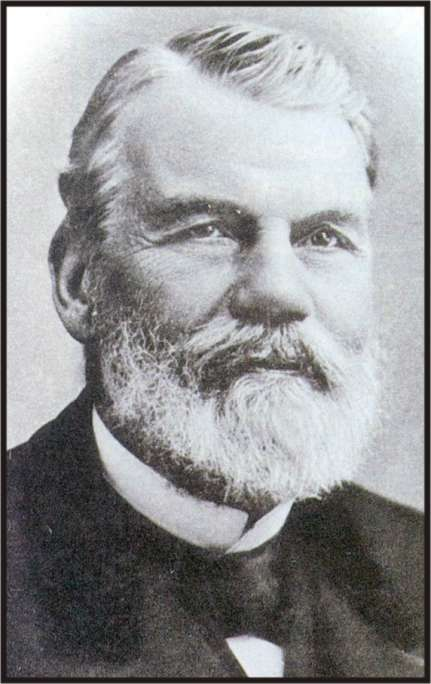
\includegraphics[width=\linewidth]{images/book3/raoult.jpg}
\end{minipage}\hfill
\begin{minipage}[t]{0.76\linewidth}\vspace{0pt}
François-Marie Raoult (1830--1901), professor of chemistry at Grenoble,
measured during the 1880s the freezing points and then the vapour pressures
of hundreds of solutions, and found that, for dilute solutions, the lowering
depends on the number of dissolved molecules and not on their nature. His
measurements became a way of weighing molecules, and supported the young
theory of ions in solution. (Photograph: public domain, Wikimedia Commons.)
\end{minipage}
\end{history}

\section{Real mixtures}

\begin{definition}[Activity coefficient]\label{def:b2:chemical-potential:activity-coefficient}
In a real mixture the \omterm{def:b2:chemical-potential:chemical-potential}{chemical potential} is written $\mu_i = \mu_i^\circ +
RT\ln a_i$ with $a_i = \gamma_i x_i$ (Raoult reference) or $a_i = \gamma_i
c_i/c^\circ$ (Henry reference). The factor $\gamma_i$ is the \emph{activity
coefficient}\index{activity coefficient}: it measures the departure from the
ideal law, and tends to 1 in the limit where the reference law holds.
\end{definition}

A coefficient above 1 means that the molecule is less stabilised by its
neighbours in the mixture than in the reference state (positive deviation, as in the figure
above); below 1, more stabilised. By Gibbs--Duhem, the coefficients of the two
constituents of a binary mixture are linked: in the one-parameter model
used for the figure, $\ln\gamma_1 = Ax_2^2$ and $\ln\gamma_2 = Ax_1^2$, and
$x_1\,\dd\ln\gamma_1 + x_2\,\dd\ln\gamma_2 = 0$ holds identically.

For ions, which interact at long range, departures appear at small
concentrations.

\begin{definition}[Ionic strength]\label{def:b2:chemical-potential:ionic-strength}
The \emph{ionic strength}\index{ionic strength} of a solution is $I =
\frac12\sum_i z_i^2\,b_i$, where $b_i$ is the molality of ion $i$ (amount per
kilogram of solvent) and $z_i$ its charge number.
\end{definition}

\begin{proposition}[Debye--Hückel limiting law]\label{prop:b2:chemical-potential:debye-huckel}
In a very dilute electrolyte solution, the mean \omterm{def:b2:chemical-potential:activity-coefficient}{activity coefficient} of the
ions of a salt obeys $\log\gamma_\pm = -A\,|z_+z_-|\sqrt{I/b^\circ}$, with $A
\approx 0.51$ for water at \qty{25}{\celsius} and $b^\circ =
\qty{1}{mol/kg}$.
\end{proposition}
\admitted

\begin{remark}[Range and origin]\label{rem:b2:chemical-potential:dh-range}
The law comes from a model in which each ion is surrounded by a diffuse
``atmosphere'' of opposite charge, which lowers its \omterm{def:b2:chemical-potential:chemical-potential}{chemical potential}; the
model is beyond this course, but its constant $A$ follows from the
permittivity and density of water and the temperature. It is accurate below
about $I = \qty{0.01}{mol/kg}$. The same ionic atmosphere slows the ions in
an electric field, and explains why the molar conductivity of a strong
electrolyte falls as $\Lambda = \Lambda^\circ - K\sqrt c$ (Kohlrausch's
square-root law) rather than staying at its limiting value: the limit of
Kohlrausch's law met in the Year 1 volume.
% ledger: epsr:H2O, rho:water.298, const:e, const:eps0, const:kB, const:NA (A computed in figdata/bachelor-2/colligative.py)
\end{remark}

\begin{example}[A centimolar salt]\label{ex:b2:chemical-potential:dh}
For sodium chloride at $b = \qty{0.010}{mol/kg}$, $I = \frac12(0.010 + 0.010)
= \qty{0.010}{mol/kg}$ and $\log\gamma_\pm = -0.51 \times 0.10$: $\gamma_\pm
= 0.89$. Already at one hundredth of a mole per kilogram, taking the
concentration for the activity is an error of 11\,\%; for a 2:2 salt such as
magnesium sulfate at the same molality, $I = 0.040$ and $\gamma_\pm = 0.62$.
\end{example}

\section{Colligative properties}

\begin{definition}[Colligative property]\label{def:b2:chemical-potential:colligative}
A \emph{colligative property}\index{colligative property} of a dilute
solution is one that depends on the amount of dissolved particles per
amount of solvent and not on their nature: the lowering of the vapour
pressure, of the freezing point, the raising of the boiling point, and the
\omterm{def:b2:chemical-potential:osmotic-pressure}{osmotic pressure}. The constants of the freezing-point and boiling-point laws
below are the \emph{cryoscopic constant}\index{cryoscopic constant} $K_f$
and the \emph{ebullioscopic constant}\index{ebullioscopic constant} $K_b$ of
the solvent.
\end{definition}

\begin{omfigure}
\begin{tikzpicture}[font=\small, >={Stealth}]
  \draw[->] (0,0) -- (8,0) node[right] {$T$};
  \draw[->] (0,0) -- (0,4.4) node[above] {$\mu$ of the solvent};
  % slopes = -S_m: the liquid, more disordered, falls faster than the solid
  \draw[omDef, very thick] (0.4,3.0) -- (7.0,2.01) node[right] {solid};
  \draw[omThm, very thick] (0.4,3.6) -- (7.6,0.72) node[right] {pure liquid};
  \draw[omThm, very thick, dashed] (0.4,3.25) -- (7.6,0.37) node[right] {solution};
  \fill (2.8,2.64) circle (1.5pt);
  \fill (1.4,2.85) circle (1.5pt);
  \draw[densely dotted] (2.8,2.64) -- (2.8,0) node[below] {$T_f^*$};
  \draw[densely dotted] (1.4,2.85) -- (1.4,0) node[below] {$T_f$};
  \draw[<->] (1.4,-0.75) -- (2.8,-0.75) node[midway, below] {$\Delta T_f$};
  \draw[<->, black!70] (5.0,1.76) -- (5.0,1.41);
  \draw[black!50] (5.0,1.58) -- (4.6,0.75) node[below, font=\scriptsize, black] {$RT\ln x_1$};
\end{tikzpicture}

{\small \omterm{def:b2:chemical-potential:chemical-potential}{Chemical potential} of the solvent against temperature (schematic,
at fixed pressure). The stable phase is the one of lowest $\mu$. Dissolving a
solute lowers the liquid's line by $RT\ln x_1 < 0$; it now meets the solid's
line at a lower temperature: the solution freezes below the pure solvent.}
\end{omfigure}

\begin{theorem}[Freezing-point depression]\label{thm:b2:chemical-potential:cryoscopy}
A dilute solution of a solute that does not enter the solid begins to freeze
at $T_f = T_f^* - \Delta T_f$, with
\[
  \Delta T_f = K_f\,b, \qquad K_f = \frac{R\,T_f^{*2}\,M_1}{\Delta_{\text{fus}}H_1} ,
\]
$b$ being the total molality of the dissolved particles and $M_1$ the molar
mass of the solvent (in \unit{kg/mol}). For finite concentrations the exact
relation for an ideal solution is $\ln x_1 = -\frac{\Delta_{\text{fus}}H_1}{R}
\left(\frac{1}{T_f} - \frac{1}{T_f^*}\right)$.
\end{theorem}

\begin{proof}
At the freezing point, pure solid solvent and solvent in the solution are in
equilibrium: $\mu_1^{\text{s}}(T) = \mu_1^{*\text{l}}(T) + RT\ln x_1$, so
$\ln x_1 = -\Delta_{\text{fus}}G_1(T)/(RT)$, with $\Delta_{\text{fus}}G_1 =
\mu_1^{*\text{l}} - \mu_1^{\text{s}}$, zero at $T_f^*$. By Gibbs--Helmholtz,
$\dd(\Delta_{\text{fus}}G_1/T)/\dd T = -\Delta_{\text{fus}}H_1/T^2$;
integrating from $T_f^*$ to $T_f$ with $\Delta_{\text{fus}}H_1$ constant gives
the exact relation. For a dilute solution, $\ln x_1 = \ln(1 - x_2) \approx
-x_2$ and $\frac1{T_f} - \frac1{T_f^*} \approx -\Delta T_f/T_f^{*2}$, so
$x_2 = \Delta_{\text{fus}}H_1\Delta T_f/(RT_f^{*2})$; finally $x_2 \approx
n_2/n_1 = b\,M_1$.
\end{proof}

\begin{proposition}[Boiling-point elevation]\label{prop:b2:chemical-potential:ebullioscopy}
A dilute solution of a non-volatile solute boils at $T_b^* + \Delta T_b$ with
$\Delta T_b = K_b\,b$, $K_b = RT_b^{*2}M_1/\Delta_{\text{vap}}H_1$.
\end{proposition}

\begin{proof}
The same, with the vapour in place of the solid: $\mu_1^{*\text{l}} +
RT\ln x_1 = \mu_1^{\text{v}}$; the solvent's line is lowered, and now meets the
vapour's line at a higher temperature.
\end{proof}

\begin{example}[Water]\label{ex:b2:chemical-potential:water-constants}
With $\Delta_{\text{fus}}H = \qty{333.4}{J/g} = \qty{6.007}{kJ/mol}$ at
\qty{273.15}{K}: $K_f = 8.314 \times 273.15^2 \times 0.018015/6007 =
\qty{1.86}{K.kg/mol}$. With $\Delta_{\text{vap}}H = \qty{40.65}{kJ/mol}$ at
\qty{373.12}{K}: $K_b = \qty{0.513}{K.kg/mol}$. Sea water, \qty{35}{g} of salt
per kilogram, counted as sodium chloride (two particles per formula):
$b = 2 \times 35/58.44/0.965 = \qty{1.24}{mol/kg}$, so the dilute law
predicts \qty{-2.3}{\celsius}, an overestimate: at this concentration the
ions are far from ideal, and sea salt is not all sodium chloride.
% ledger: dfus:H2O, tfus:H2O, dvap:H2O.nbp, tb:H2O.atm, sea:salinity (computed in figdata/bachelor-2/colligative.py)
\end{example}

\begin{definition}[Semipermeable membrane, osmotic pressure]\label{def:b2:chemical-potential:osmotic-pressure}
A \emph{semipermeable membrane}\index{semipermeable membrane} lets the
solvent through and not the solute. When it separates a solution from the
pure solvent, the solvent flows into the solution; the \emph{osmotic
pressure}\index{osmotic pressure} $\Pi$ is the excess pressure that must be
applied to the solution to stop that flow.
\end{definition}

\begin{theorem}[van 't Hoff's osmotic law]\label{thm:b2:chemical-potential:osmosis}
For a dilute solution, $\Pi = c\,RT$, where $c$ is the total concentration of
solute particles.
\end{theorem}

\begin{proof}
At equilibrium the solvent has the same \omterm{def:b2:chemical-potential:chemical-potential}{chemical potential} on both sides:
$\mu_1^*(T, p) = \mu_1^*(T, p + \Pi) + RT\ln x_1$. Since $(\partial\mu_1^*/
\partial p)_T = V_{m,1}$, nearly constant for a liquid, $\mu_1^*(T, p + \Pi) -
\mu_1^*(T, p) = \Pi V_{m,1}$, so $\Pi V_{m,1} = -RT\ln x_1 \approx RT x_2
\approx RT\,n_2/n_1$. With $n_1V_{m,1} \approx V$ (dilute), $\Pi = n_2RT/V$.
\end{proof}

\begin{omfigure}
\begin{tikzpicture}[font=\small, >={Stealth}]
  \begin{scope}
    \clip (-0.85,2.8) -- (-0.85,0.85) arc[start angle=180, end angle=360,
      radius=0.85] -- (0.85,2.8) -- (0.55,2.8) -- (0.55,0.85)
      arc[start angle=0, end angle=-180, radius=0.55] -- (-0.55,2.8) -- cycle;
    \fill[omDef!18] (-1,0) rectangle (0,1.6);
    \fill[omThm!22] (0,0) rectangle (1,2.3);
  \end{scope}
  \pic at (0,0) {utube={0}{white}};
  \draw[very thick, dashed] (0,-0.05) -- (0,0.36);
  \node[left] at (-1.0,1.2) {pure water};
  \node[right] at (1.0,0.9) {solution};
  \draw[densely dotted] (-0.55,1.6) -- (1.55,1.6);
  \draw[densely dotted] (0.85,2.3) -- (1.55,2.3);
  \draw[<->, thick] (1.45,1.6) -- (1.45,2.3) node[midway, right] {$h$, with $\Pi = \rho g h$};
  \draw (0,0.12) -- (0.6,-0.5) node[below right] {semipermeable membrane};
  \draw[->, omDef, thick] (-0.75,0.4) to[bend right=30] (-0.25,0.12);
\end{tikzpicture}

{\small Osmosis in a U-tube. Water passes through the membrane into the
solution until the extra hydrostatic pressure of the higher column equals
the \omterm{def:b2:chemical-potential:osmotic-pressure}{osmotic pressure}; then the \omterm{def:b2:chemical-potential:chemical-potential}{chemical potentials} of water on the two sides
are equal.}
\end{omfigure}

\begin{method}[Molar mass by a colligative property]\label{met:b2:chemical-potential:molar-mass}
\begin{enumerate}
  \item Dissolve a known mass $m_2$ of the substance in a known mass $m_1$
        of solvent (or a known volume $V$ of solution).
  \item Measure $\Delta T_f$ (or $\Delta T_b$, or $\Pi$).
  \item Deduce the molality $b = \Delta T_f/K_f$ (or $c = \Pi/RT$), then $n_2 =
        b\,m_1$ (or $cV$) and $M_2 = m_2/n_2$; divide by the number of
        particles per formula if the substance dissociates.
\end{enumerate}
Osmometry suits large molecules (proteins, polymers): a few grams per litre
of a protein of \qty{60}{kg/mol} give a few hundred pascals, millimetres of
water, but a freezing-point change of only a few thousandths of a kelvin.
\end{method}

\section{Exercises}

\begin{exercise}[$\star$]\label{exo:b2:chemical-potential:1}
Use the tangent construction on the figure of the molar volume (model
mixture) at $x_2 = 0.4$ to read $\bar V_1$ and $\bar V_2$, and check that
$x_1\bar V_1 + x_2\bar V_2$ is the molar volume of the mixture.
\end{exercise}

\begin{exercise}[$\star$]\label{exo:b2:chemical-potential:2}
At \qty{25}{\celsius} the vapour pressure of water is \qty{3.17}{kPa}.
Compute, by \omterm{thm:b2:chemical-potential:raoult}{Raoult's law}, the vapour pressure above a solution of
\qty{1.00}{mol} of sucrose (non-volatile) in \qty{1.00}{kg} of water.
% ledger: pvap:H2O.298
\end{exercise}

\begin{exercise}[$\star$]\label{exo:b2:chemical-potential:3}
Compute the concentration of dioxygen dissolved in water in equilibrium with
air at \qty{1.013}{bar} and \qty{25}{\celsius} ($H(\ce{O2}) =
\qty{1.3e-5}{mol/(m^3.Pa)}$, \qty{20.95}{\percent} of dioxygen), in
\unit{mol/L} and \unit{mg/L}.
% ledger: henry:O2, air:O2
\end{exercise}

\begin{exercise}[$\star$]\label{exo:b2:chemical-potential:4}
For \ce{N2(g) + 3H2(g) <=> 2NH3(g)} at \qty{298}{K}, $\Delta_r G^\circ =
\qty{-32.8}{kJ/mol}$. Compute $\Delta_r G$ in a mixture where
$p(\ce{N2}) = \qty{1.0}{bar}$, $p(\ce{H2}) = \qty{0.010}{bar}$ and
$p(\ce{NH3}) = \qty{1.0}{bar}$, and say which way the reaction goes.
\end{exercise}

\begin{exercise}[$\star\star$]\label{exo:b2:chemical-potential:5}
In a binary mixture, the \omterm{def:b2:chemical-potential:partial-molar}{partial molar volume} of constituent 1 changes by
$\dd\bar V_1 = \qty{-0.30}{mL/mol}$ when $x_2$ goes from 0.30 to 0.31. Using
Gibbs--Duhem, find $\dd\bar V_2$.
\end{exercise}

\begin{exercise}[$\star\star$]\label{exo:b2:chemical-potential:6}
Physiological saline contains \qty{9.0}{g} of sodium chloride per litre.
Compute its \omterm{def:b2:chemical-potential:osmotic-pressure}{osmotic pressure} at \qty{37}{\celsius}, taking the salt as fully
dissociated, and explain why red blood cells keep their shape in it but swell
and burst in pure water.
\end{exercise}

\begin{exercise}[$\star\star$]\label{exo:b2:chemical-potential:7}
A solution of \qty{2.00}{g} of a protein in \qty{100.0}{mL} of water has an
\omterm{def:b2:chemical-potential:osmotic-pressure}{osmotic pressure} of \qty{0.825}{kPa} at \qty{25}{\celsius}. Compute the molar
mass of the protein, and the freezing-point depression of this solution.
\end{exercise}

\begin{exercise}[$\star\star$]\label{exo:b2:chemical-potential:8}
Compute the \omterm{def:b2:chemical-potential:ionic-strength}{ionic strength} and the mean \omterm{def:b2:chemical-potential:activity-coefficient}{activity coefficients} (limiting law)
of: (a) \qty{1.0e-3}{mol/kg} sodium chloride; (b) \qty{1.0e-3}{mol/kg}
calcium chloride; (c) \qty{1.0e-3}{mol/kg} magnesium sulfate.
\end{exercise}

\begin{exercise}[$\star\star$]\label{exo:b2:chemical-potential:9}
A solution of \qty{1.50}{g} of an unknown non-volatile, non-dissociating
compound in \qty{50.0}{g} of water freezes at \qty{-0.310}{\celsius}. Compute
its molar mass.
\end{exercise}

\begin{exercise}[$\star\star\star$]\label{exo:b2:chemical-potential:10}
Show that in the one-parameter model $\ln\gamma_1 = Ax_2^2$, $\ln\gamma_2 =
Ax_1^2$, the Gibbs--Duhem relation holds, and that the \omterm{prop:b2:chemical-potential:henry}{Henry constant} of
constituent 1 is $k_{H,1} = p_1^*\mathrm e^A$. For $A = 1.1$, by what factor
does Henry's slope exceed Raoult's?
\end{exercise}

\begin{exercise}[$\star\star\star$]\label{exo:b2:chemical-potential:11}
Explain why a colligative law needs (a) a non-volatile solute for the
boiling-point elevation, and (b) a solute that does not enter the solid for
the freezing-point depression. What happens to the freezing point of a
solvent whose solute forms an ideal solid solution with it in the same
proportion as in the liquid?
\end{exercise}

\begin{exercise}[$\star\star\star$]\label{exo:b2:chemical-potential:12}
A thermometer reads to \qty{0.01}{K}. Compute the smallest molality of a
non-dissociating solute detectable in water by cryoscopy and by
ebullioscopy, and the corresponding \omterm{def:b2:chemical-potential:osmotic-pressure}{osmotic pressure} at \qty{25}{\celsius}.
Which method is the most sensitive, and why are osmometers used for polymers?
\end{exercise}

\section{Problem: The Radiator in Winter}

\begin{problem}[{Weekend problem --- an \omterm{def:b2:chemical-potential:ideal-mixture}{ideal mixture} of water and
ethane-1,2-diol, the cryoscopic law and its constant, the freezing of a
coolant, and how much diol keeps an engine liquid at \qty{-20}{\celsius}}]
\label{pb:b2:chemical-potential:1}
The coolant of an engine is a mixture of water and ethane-1,2-diol
(\ce{HOCH2CH2OH}, $M = \qty{62.07}{g/mol}$, boiling point \qty{197}{\celsius},
non-volatile here). Water: $M = \qty{18.015}{g/mol}$, freezing point
\qty{273.15}{K}, enthalpy of fusion \qty{333.4}{J/g}, boiling point
\qty{373.12}{K} under \qty{1.013}{bar}, enthalpy of vaporisation
\qty{40.65}{kJ/mol}, vapour pressure \qty{3.17}{kPa} at \qty{25}{\celsius}.
The mixture is taken as ideal.
% ledger: tb:glycol, dfus:H2O, tfus:H2O, tb:H2O.atm, dvap:H2O.nbp, pvap:H2O.298

\medskip
\noindent\textbf{Part I --- The mixture.}
\begin{enumerate}
  \item Write the \omterm{def:b2:chemical-potential:chemical-potential}{chemical potential} of water in an \omterm{def:b2:chemical-potential:ideal-mixture}{ideal mixture}.
  \item A coolant contains \qty{30}{\percent} of diol by mass. Compute the
        amounts of diol and water in \qty{100}{g}, and the mole fraction of
        water.
  \item Compute the vapour pressure of water above this coolant at
        \qty{25}{\celsius}.
  \item Compute the molality of the diol.
  \item Why is the diol's own vapour pressure neglected?
\end{enumerate}

\medskip
\noindent\textbf{Part II --- The cryoscopic law.}
\begin{enumerate}[resume]
  \item Write the equality of \omterm{def:b2:chemical-potential:chemical-potential}{chemical potentials} at the freezing point of
        the coolant, the solid being pure ice.
  \item Using the Gibbs--Helmholtz relation, derive $\ln x_1 =
        -\frac{\Delta_{\text{fus}}H}{R}\left(\frac1{T_f} - \frac1{T_f^*}\right)$.
  \item Linearise it for a dilute solution and obtain $\Delta T_f = K_f b$.
  \item Compute the molar enthalpy of fusion of water and $K_f$.
  \item What assumption about the enthalpy of fusion did the integration
        make?
\end{enumerate}

\medskip
\noindent\textbf{Part III --- Freezing.}
\begin{enumerate}[resume]
  \item Compute the freezing point of the \qty{30}{\percent} coolant with the
        dilute law.
  \item Compute it with the exact ideal relation.
  \item Which result do you trust more, and why are both only estimates for a
        real coolant?
  \item At the freezing point, what crystallises?
  \item Cooled further, the remaining liquid becomes richer in diol. Explain
        why ice keeps forming at lower and lower temperatures.
\end{enumerate}

\medskip
\noindent\textbf{Part IV --- Boiling, and the winter target.}
\begin{enumerate}[resume]
  \item Compute $K_b$ of water.
  \item Compute the boiling-point elevation of the \qty{30}{\percent} coolant
        at \qty{1.013}{bar}.
  \item The radiator is pressurised to \qty{2.0}{bar}. Using the
        Clausius--Clapeyron relation of physics with the enthalpy of
        vaporisation above, estimate the boiling point of pure water at
        \qty{2.0}{bar}.
  \item Which matters more for the summer, the cap or the diol?
  \item For a coolant liquid down to \qty{-20}{\celsius}, compute the mole
        fraction of water required by the exact ideal relation.
  \item Convert it into a mass fraction of diol.
  \item Compute the mass fraction that the dilute law would have given, and
        explain the difference.
  \item State the mass fraction of diol that keeps the coolant liquid down to
        \qty{-20}{\celsius} in the ideal-mixture model.
\end{enumerate}
\end{problem}
